% exercise sheet with header on every page for math or close subjects
\documentclass[12pt]{article}
\usepackage[utf8]{inputenc}
\usepackage{latexsym}
\usepackage{multicol}
\usepackage{fancyhdr}
\usepackage{amsfonts}
\usepackage{amsmath}
\usepackage{amssymb}
\usepackage{enumerate}
\usepackage{listings}
\usepackage{graphicx}
\usepackage[parfill]{parskip}

% Shortcuts for bb, frak and cal letters
\newcommand{\E}{\mathbb{E}}
\newcommand{\V}{\mathbb{V}}
\renewcommand{\P}{\mathbb{P}}
\newcommand{\N}{\mathbb{N}}
\newcommand{\R}{\mathbb{R}}
\newcommand{\C}{\mathbb{C}}
\newcommand{\Z}{\mathbb{Z}}
\newcommand{\Pfrak}{\mathfrak{P}}
\newcommand{\Pfrac}{\mathfrak{P}}
\newcommand{\Bfrac}{\mathfrak{P}}
\newcommand{\Bfrak}{\mathfrak{B}}
\newcommand{\Fcal}{\mathcal{F}}
\newcommand{\Ycal}{\mathcal{Y}}
\newcommand{\Bcal}{\mathcal{B}}
\newcommand{\Acal}{\mathcal{A}}

% formating
\topmargin -3.5cm
\textheight 22cm
\textwidth 16.0 cm
\oddsidemargin -0.1cm

% Fancy Header on every Page
\pagestyle{fancy}
\lhead{\textbf{Embedded Systems Problem Set C}}
\rhead{Daniel Schäfer (2549458)\\ Rafael Dewes (2548365)\\ Kevin M\"uller (2550062)}
\renewcommand{\headrulewidth}{1.2pt}
\setlength{\headheight}{110pt}

\begin{document}
\pagenumbering{gobble}
\lstset{language=C++}

\section*{Problem C1}
I selected the LDF (Latest Deadline First) scheduler to schedule this task with , which results in the following:
\begin{figure}[h]
	\centering
	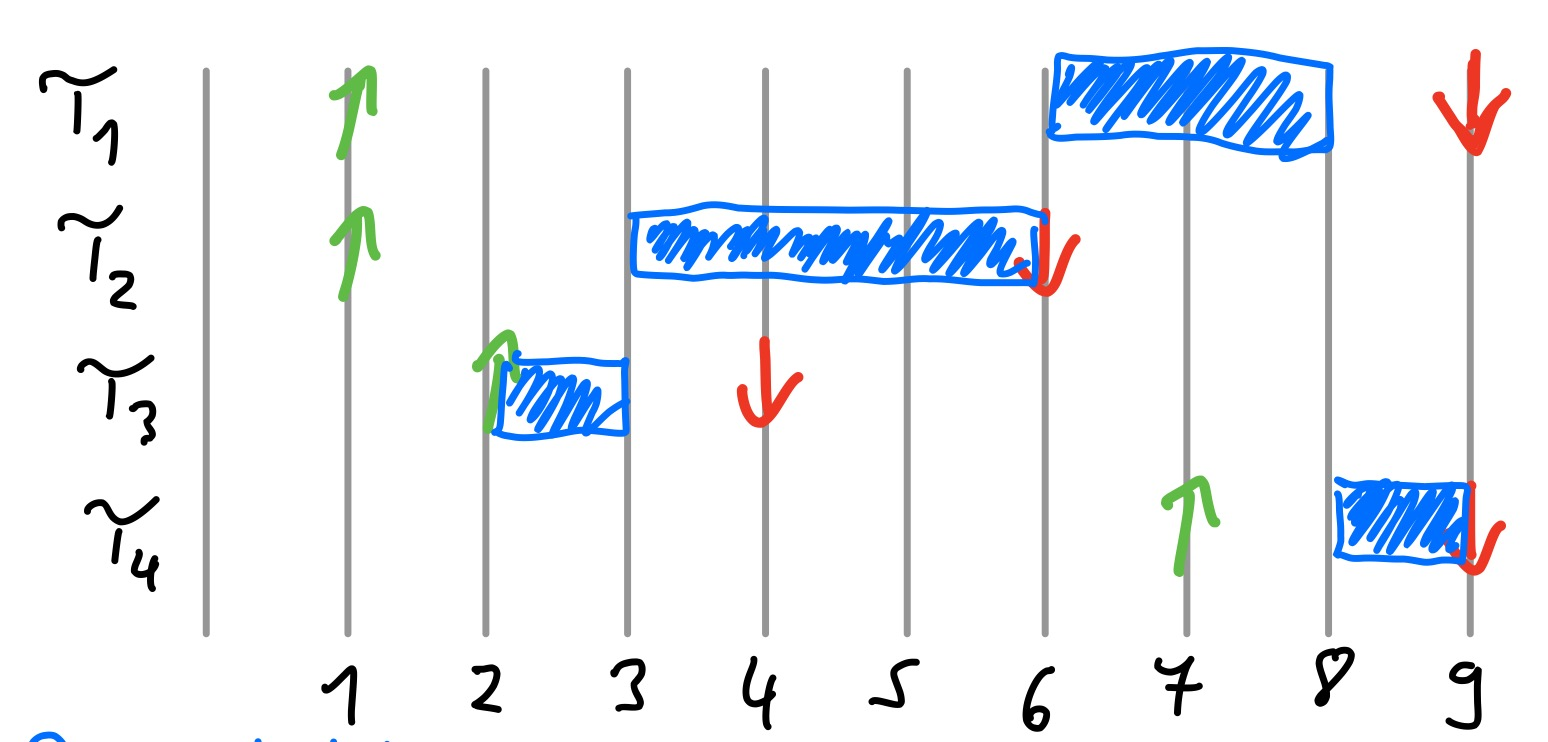
\includegraphics[scale = 0.25]{figures/c1}\\
\end{figure}

\newpage
\section*{Problem C2}
\begin{itemize}
	\item
	  for $\Gamma$ I calculate the Utilization in timeframe $t=12$.
		$$ U = \frac{6 * C(\tau_1) + 2 * C(\tau_2) + 1 * C(\tau_3)}{12} = \frac{11}{12}$$
		\begin{figure}[h]
			\centering
			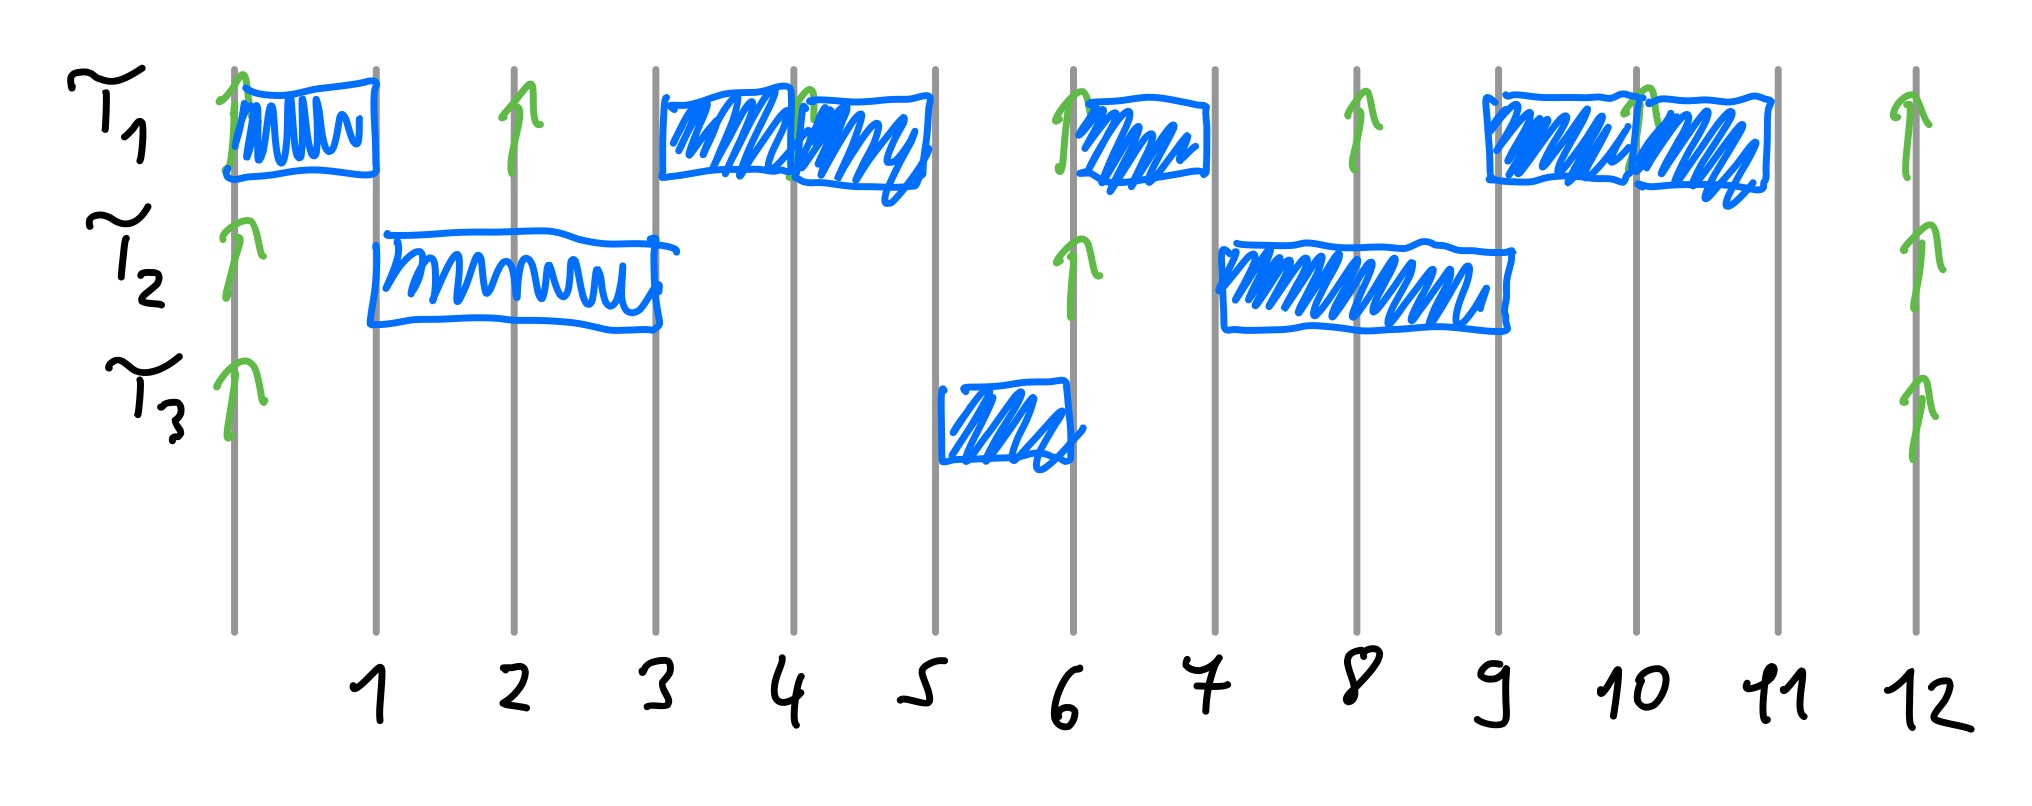
\includegraphics[scale = 0.2]{figures/c2_1}
			\caption{The RM-Schedule for $\Gamma$ for $t=12$}
		\end{figure}

		\begin{figure}[h]
			\centering
			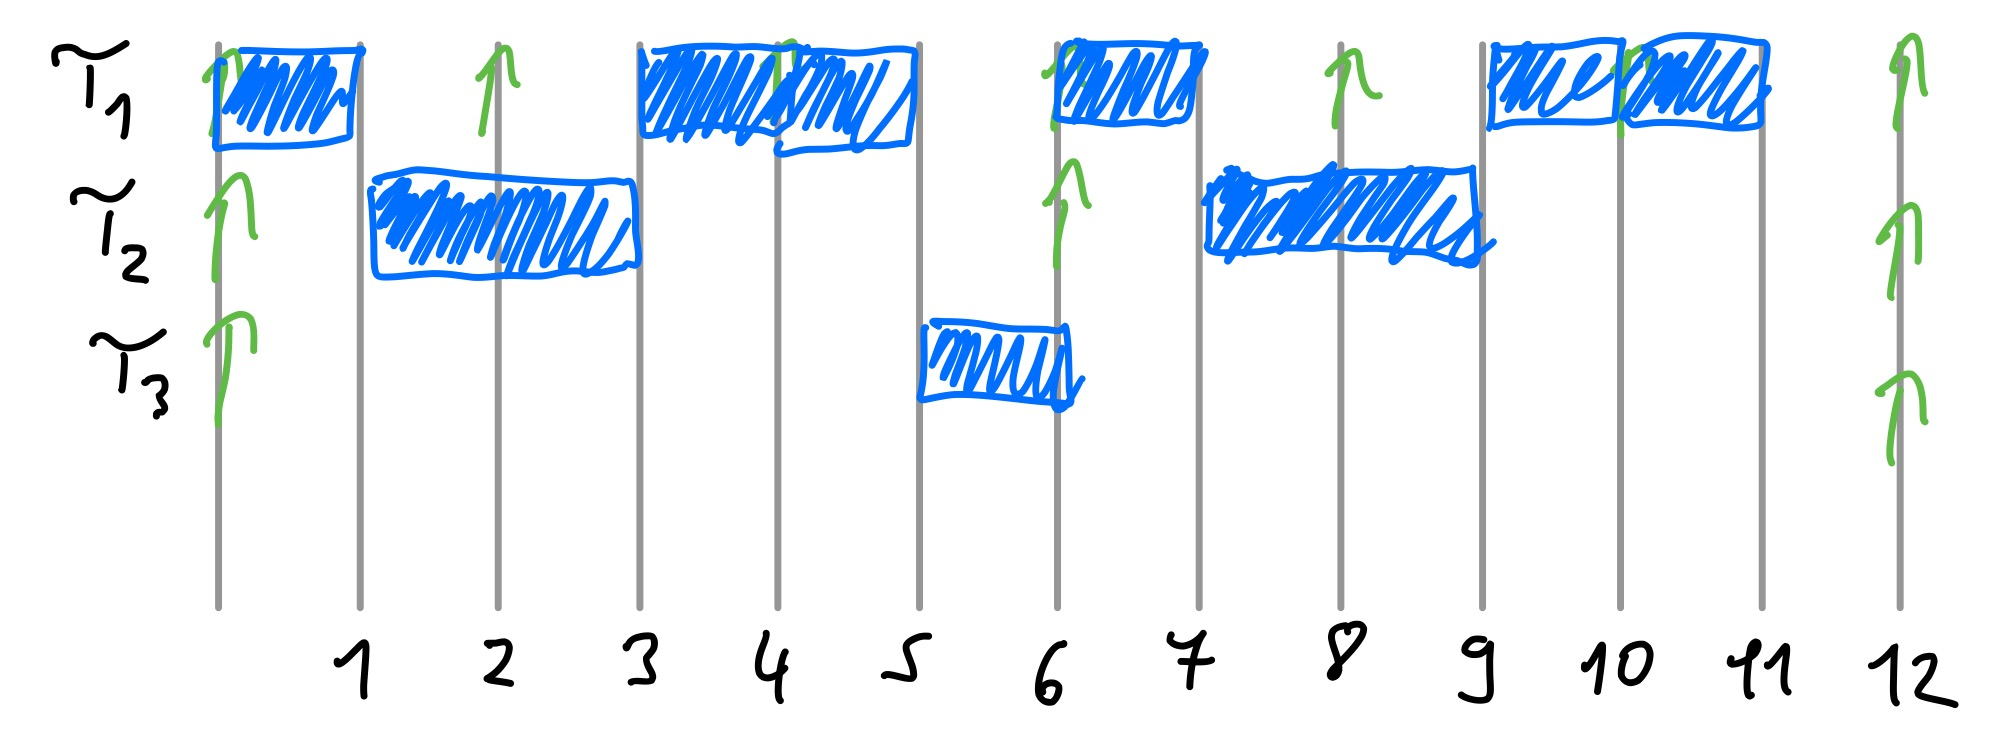
\includegraphics[scale = 0.2]{figures/c2_2}
			\caption{The EDF-Schedule for $\Gamma$ for $t=12$}
		\end{figure}
  \item
    for $\Delta$ I calculate the Utilization in timeframe $t=24$.
		$$U = \frac{1 * C(\tau_4) + 2 * C(\tau_3) + 3 * C(\tau_2) + 4 * C(\tau_1)}{24} = \frac{1 + 6 + 6 + 12}{24} = \frac{25}{24}$$

		Utilization $\frac{25}{24} > 1$, means that this task can not be completed in any scheduler on a single care as it is not feasible.
\newpage
	\item
		for $\Lambda$ I calculate the Utilization in timeframe $t=40$.
		$$U = \frac{1 * C(\tau_4) + 5 * C(\tau_3) + 8 * C(\tau_2) + 20 * C(\tau_1)}{40} = \frac{2 + 10 + 8 + 20}{40} = \frac{40}{40} = 100 \%$$

		\begin{figure}[h]
		\centering
		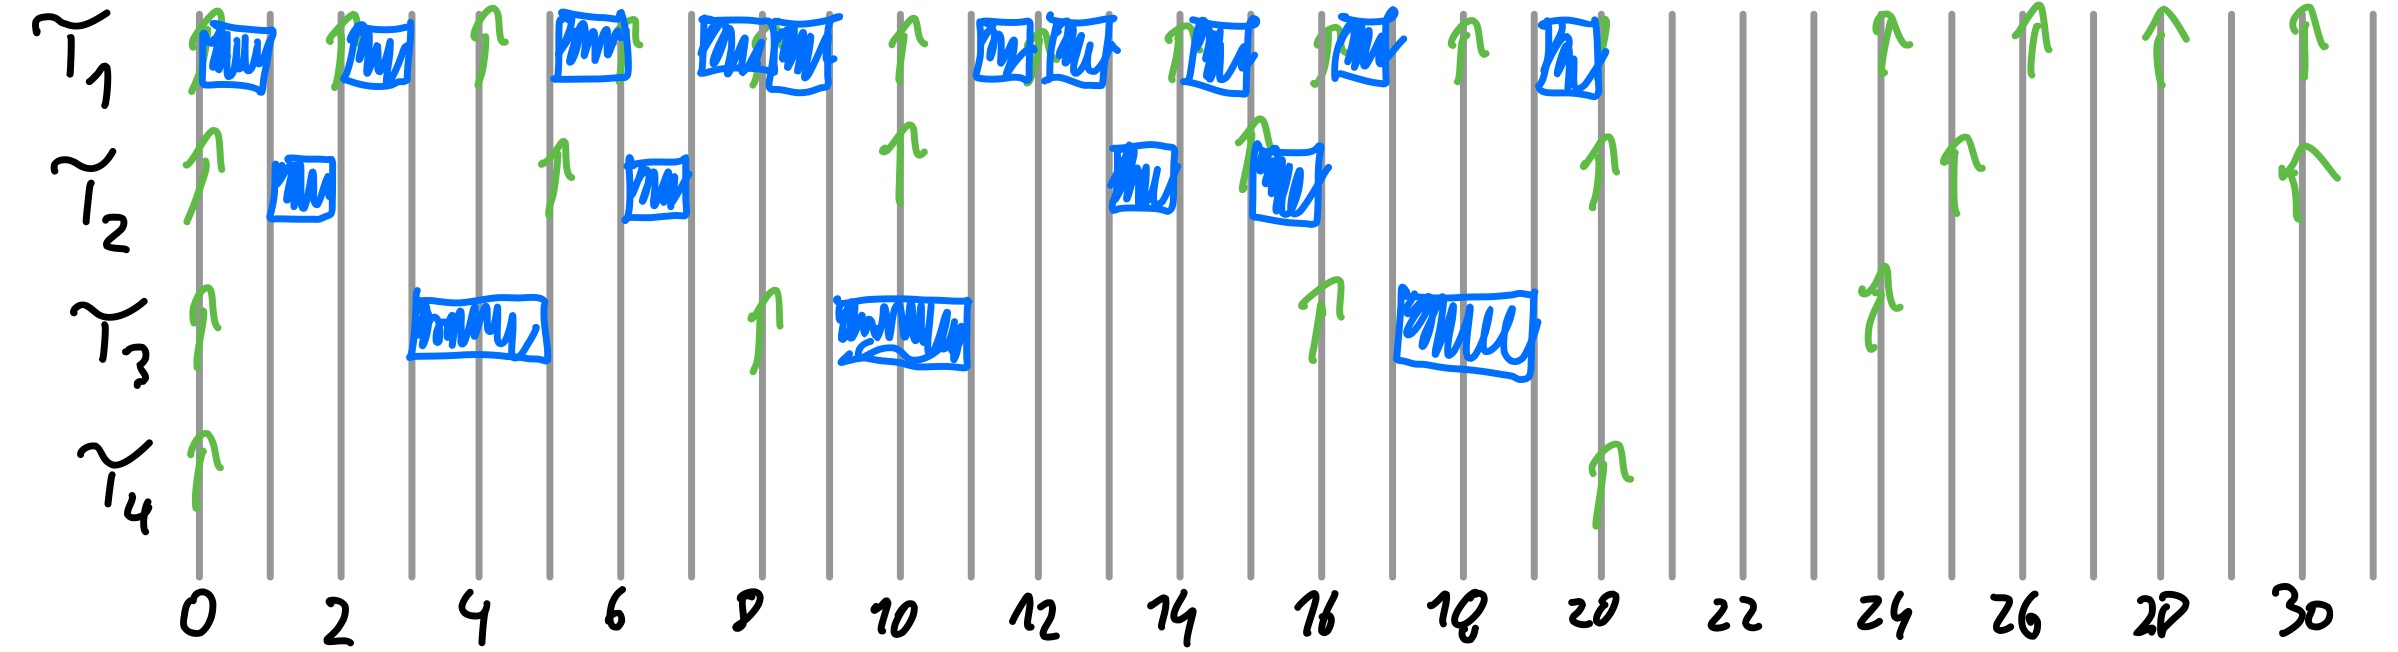
\includegraphics[scale = 0.2]{figures/c2_3}
		\caption{The RM-Schedule for $\Lambda$}
		\end{figure}

		\begin{figure}[h]
		\centering
		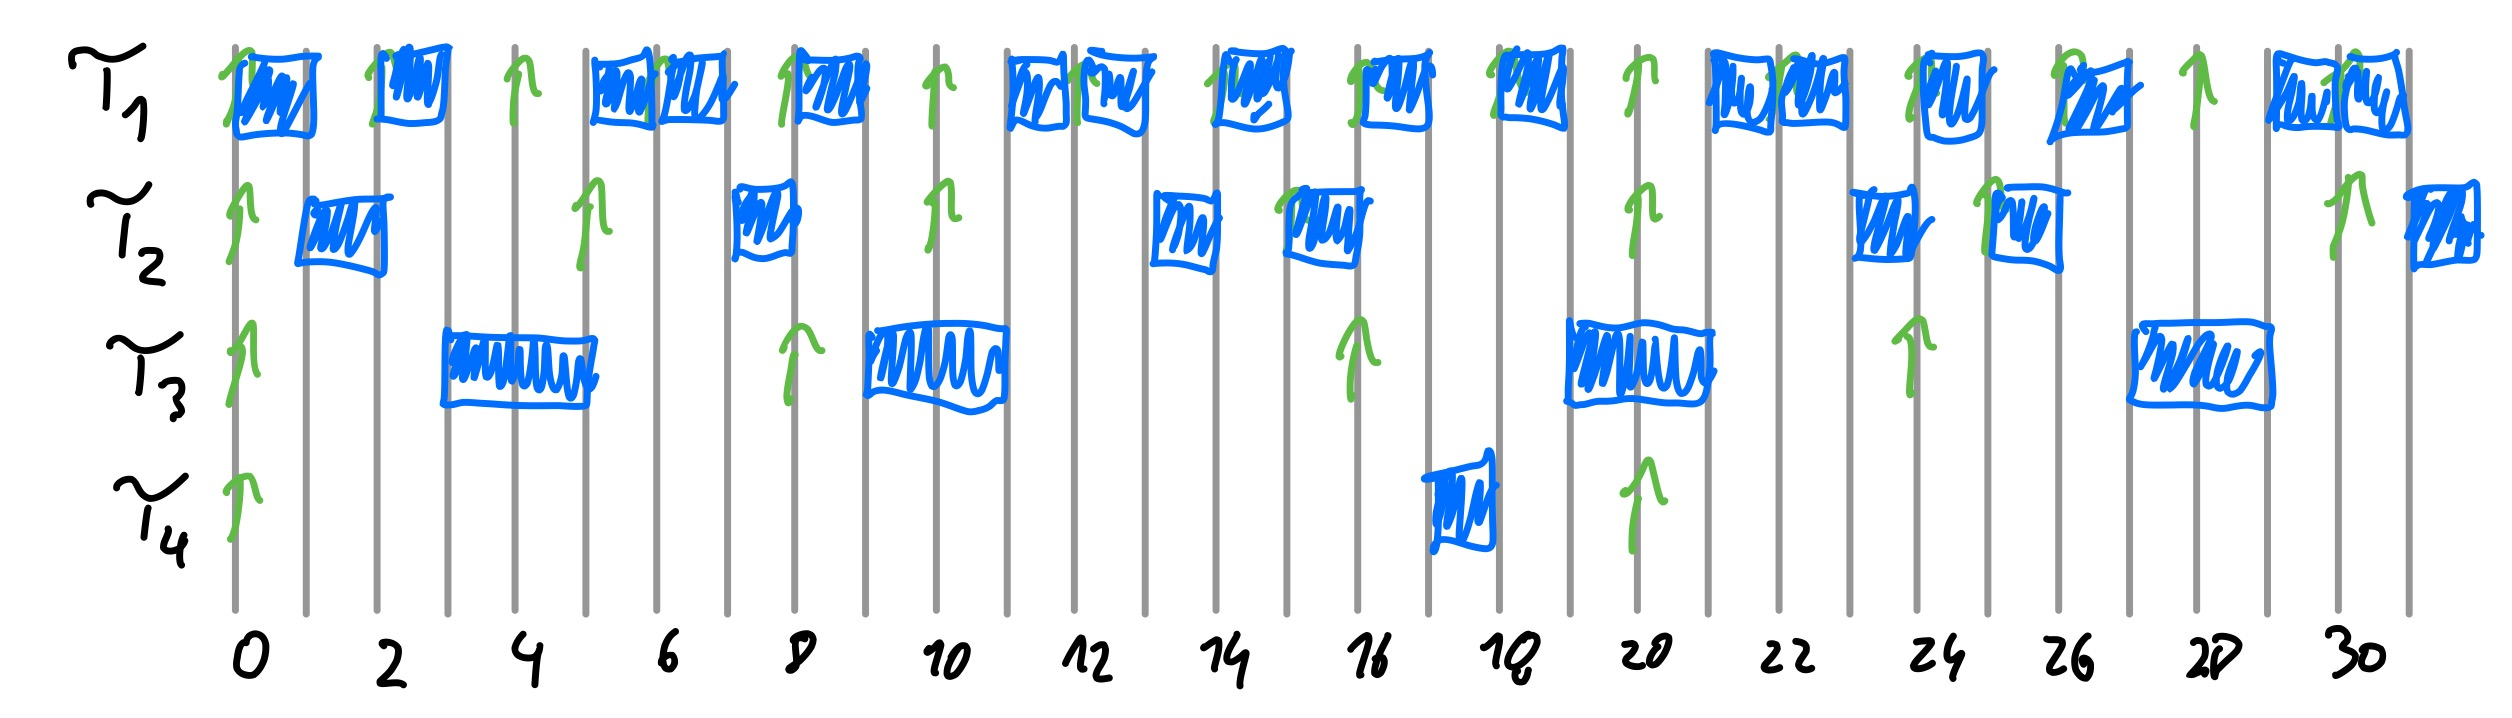
\includegraphics[scale = 0.15]{figures/c2_4}
		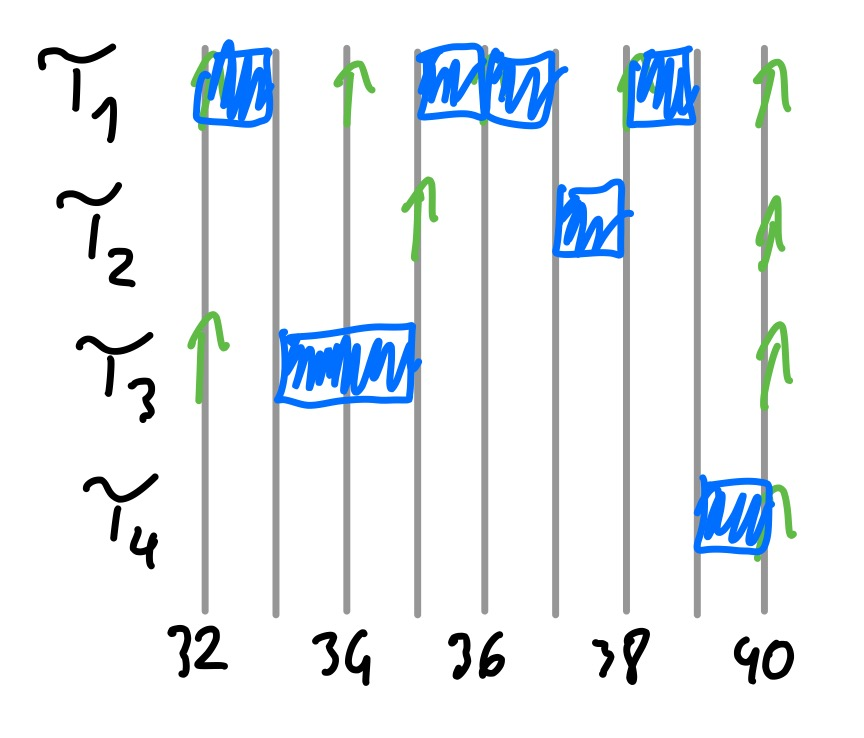
\includegraphics[scale = 0.15]{figures/c2_5}
		\caption{The EDF-Schedule for $\Lambda$}
		\end{figure}


\section*{Problem C3}
% TODO

\section*{Problem C4}
% TODO

\end{document}
